%%%%%%%%%%%%%%%%%%%%%%%%%%%%%%%%%%%%%%%%%
% Journal Article
% LaTeX Template
% Version 1.4 (15/5/16)
%
% This template has been downloaded from:
% http://www.LaTeXTemplates.com
%
% Original author:
% Frits Wenneker (http://www.howtotex.com) with extensive modifications by
% Vel (vel@LaTeXTemplates.com)
%
% License:
% CC BY-NC-SA 3.0 (http://creativecommons.org/licenses/by-nc-sa/3.0/)
%
%%%%%%%%%%%%%%%%%%%%%%%%%%%%%%%%%%%%%%%%%

%----------------------------------------------------------------------------------------
%   PACKAGES AND OTHER DOCUMENT CONFIGURATIONS
%----------------------------------------------------------------------------------------

\documentclass[twoside,twocolumn]{article}

\usepackage{blindtext} % Package to generate dummy text throughout this template
\usepackage{amsmath}
\usepackage[sc]{mathpazo} % Use the Palatino font
\usepackage[T1]{fontenc} % Use 8-bit encoding that has 256 glyphs
\linespread{1.05} % Line spacing - Palatino needs more space between lines
\usepackage{microtype} % Slightly tweak font spacing for aesthetics

\usepackage[english]{babel} % Language hyphenation and typographical rules

\usepackage[hmarginratio=1:1,top=32mm,columnsep=20pt]{geometry} % Document margins
\usepackage[hang, small,labelfont=bf,up,textfont=it,up]{caption} % Custom captions under/above floats in tables or figures
\usepackage{booktabs} % Horizontal rules in tables

\usepackage{lettrine} % The lettrine is the first enlarged letter at the beginning of the text

\usepackage{enumitem} % Customized lists
\setlist[itemize]{noitemsep} % Make itemize lists more compact

\usepackage{abstract} % Allows abstract customization
\renewcommand{\abstractnamefont}{\normalfont\bfseries} % Set the "Abstract" text to bold
\renewcommand{\abstracttextfont}{\normalfont\small\itshape} % Set the abstract itself to small italic text

\usepackage{titlesec} % Allows customization of titles
\renewcommand\thesection{\Roman{section}} % Roman numerals for the sections
\renewcommand\thesubsection{\roman{subsection}} % roman numerals for subsections
\titleformat{\section}[block]{\large\scshape\centering}{\thesection.}{1em}{} % Change the look of the section titles
\titleformat{\subsection}[block]{\large}{\thesubsection.}{1em}{} % Change the look of the section titles

\usepackage{fancyhdr} % Headers and footers
\pagestyle{fancy} % All pages have headers and footers
\fancyhead{} % Blank out the default header
\fancyfoot{} % Blank out the default footer
\fancyhead[C]{Music Generation $\bullet$ December 2018 $\bullet$ Tang, Xu, Xu} % Custom header text
\fancyfoot[RO,LE]{\thepage} % Custom footer text

\usepackage{titling} % Customizing the title section

\usepackage{hyperref} % For hyperlinks in the PDF
\usepackage{url}
\usepackage{graphicx}
\graphicspath{ {./images/}}

%----------------------------------------------------------------------------------------
%   TITLE SECTION
%----------------------------------------------------------------------------------------

\setlength{\droptitle}{-4\baselineskip} % Move the title up

\pretitle{\begin{center}\Huge\bfseries} % Article title formatting
\posttitle{\end{center}} % Article title closing formatting
\title{Music Generation with LSTMs} % Article title
\author{%
\textsc{Joyce Xu} \\[1ex] % Your name
\normalsize Stanford University \\ % Your institution
\normalsize \href{mailto:jexu@stanford.edu}{jexu@stanford.edu} % Your email address
\and % Uncomment if 2 authors are required, duplicate these 4 lines if more
\textsc{Sam Xu} \\[1ex] % Second author's name
\normalsize Stanford University \\ % Second author's institution
\normalsize \href{mailto:samx}{samx@stanford.edu} % Second author's email address
\and % Uncomment if 2 authors are required, duplicate these 4 lines if more
\textsc{Eric Tang} \\[1ex] % Second author's name
\normalsize Stanford University \\ % Second author's institution
\normalsize \href{mailto:etang21@stanford.edu}{etang21@stanford.edu} % Second author's email address
}
\date{\today} % Leave empty to omit a date

%----------------------------------------------------------------------------------------

\renewcommand{\maketitlehookd}{%
\begin{abstract}
\noindent
Music composition is an extremely creative task, and consequently very difficult for AI models to successfully perform. In this paper, we explore several techniques for generating music using deep neural networks, specifically Long Short-Term Memory networks (LSTMs) and attention-based LSTMs. In a human evaluation of musical quality, our LSTM-generated compositions outperformed a composition generated using logistic regression techniques, but failed to match the quality of human-generated compositions. We briefly discuss potential techniques to improve the quality of our LSTM compositions.
\end{abstract}
}

%----------------------------------------------------------------------------------------

\begin{document}

% Print the title
\maketitle

%----------------------------------------------------------------------------------------
%   ARTICLE CONTENTS
%----------------------------------------------------------------------------------------

\section{Introduction}

Music exhibits both short-term structure, such as the relation between successive chords and notes, and long-term structure, such as a song's overall key, tempo, and melody. Previous results in music generation have seen limited success, largely due to difficulties in capturing music's complex long-term structure. Recently, however, the use of novel network architectures, such as Long Short-Term Memory networks (LSTMs) and variational autoencoders (VAEs) have opened new possibilities for music generation \cite{lstm-vae}.

In this paper, we train several models to take in a sequence of single notes (the melody) and predict the subsequent note in the melody. For each model, our input is the sequence of previous notes in the melody, with each note's pitch encoded as a one-hot vector. Our model then outputs a one-hot vector corresponding to the most plausible subsequent note of the melody. We use each model to compose music by feeding the model a seed sequence of notes, then repeatedly predicting the subsequent note and appending it to the composition. We develop and compare three models: logistic regression, a standard LSTM, and an LSTM utilizing attention. We find that the LSTM and attention LSTM significantly outperform our baseline, but still fall well short of human-level composition.

\section{Related Work}
Early attempts to compose music using neural networks utilized Recurrent Neural Networks (RNNs) to predict successive notes in a composition, concatenating these predicted notes to form a melody. Unfortunately, RNN models failed to sufficiently model long-term structures in music, typically suffering from "a lack of global coherence" \cite{Mozer}. Early work by Eck and Schmidhuber overcame these challenges by using LSTMs to model sequences of notes, finding better long-term structure in the resulting compositions of blues melodies \cite{eck}. More recent works have used Variational Autoencoders (VAEs) to model, reconstruct, and compose sequences of musical notes. In particular, Roberts et al. find high performance using Hierarchical VAEs, which significantly outperform flat VAEs in listener evaluations \cite{lstm-vae}.

Recent papers have also utilized neural network models, such as LSTMs, to extract embedded vector representations for notes in each sequence. Huang and Wu train LSTM models on several datasets of classical music and extract the learned vector embeddings from their models \cite{huang-wu}. They then use PCA and t-sne visualization techniques to visualize the learned embeddings; their visualizations display clear structure in the learned embeddings, further affirming the power of LSTM models. Madjiheurem et al. take a similar approach by using a sequence-to-sequence LSTM model to predict successive chords, and taking the LSTM's vector encoding of an input chord as the vector embedding for a given chord \cite{Madjiheurem}. They find that this sequence-to-sequence model outperforms bilinear and autoregressive models, while also producing more sensible embedded representations.

%------------------------------------------------

\section{Dataset}

We begin our exploration with two datasets: one of 26 Beethoven compositions, and the other of 18 Mozart compositions, both stored in the popular MIDI format. MIDI files contain information about each note's pitch and duration in a score. This gives us a rich starting place for our exploration. Both collections were sourced from a repository of classical piano scores in MIDI format \cite{classical-piano-midi}. We then used the music21 library, developed at music21, to process our MIDI files into sequences of pitches \cite{music21}. We tackled the simplified problem of composing melodies without chords, by taking just one pitch from each chord in the existing melodies. The resulting distribution of extracted notes is displayed below.

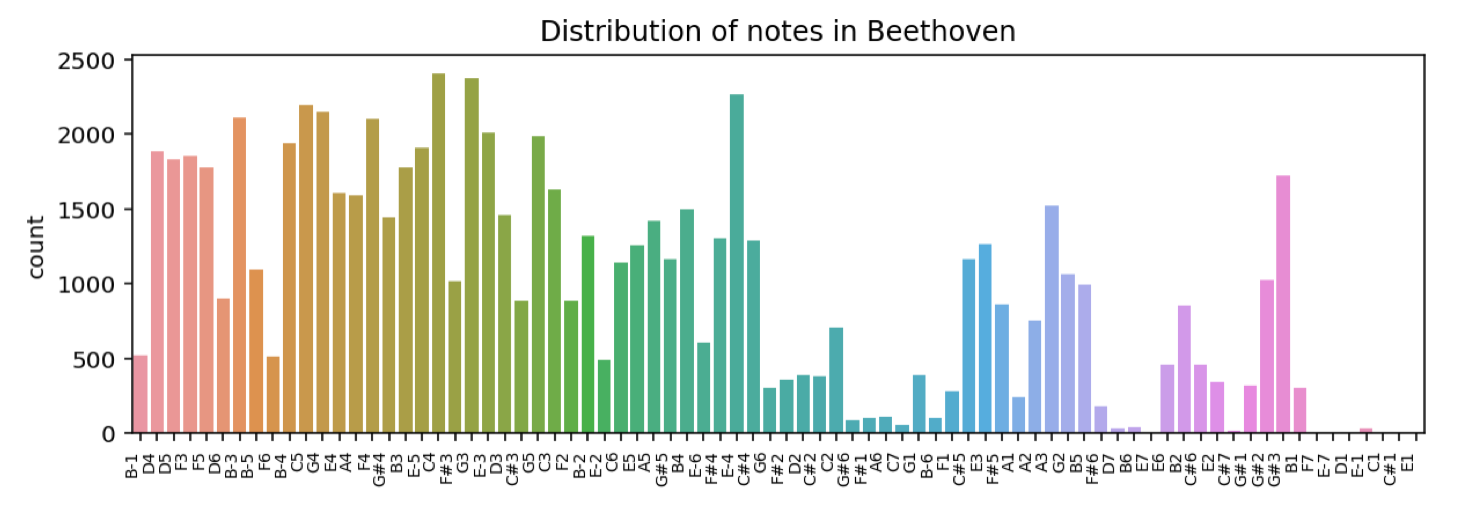
\includegraphics[width = 0.4\textwidth]{note-distribution}

We then featurized the notes/chords as sequences of multi-hot vectors, where we first mapped all unique pitches in song to an index, then transformed individual notes to one-hot vector, and chords to multi-hot vectors (based on pitches).

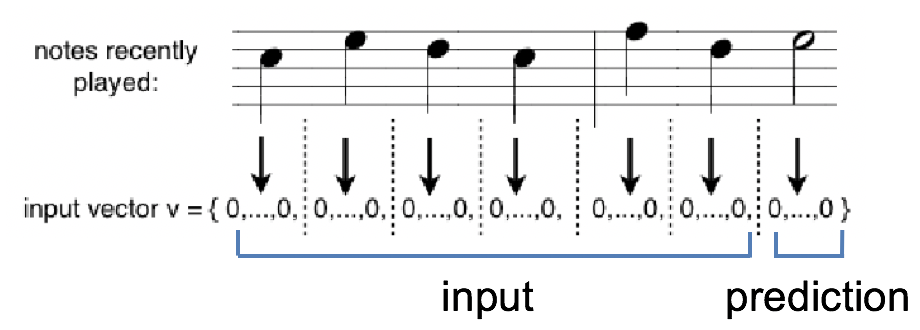
\includegraphics[width = 0.4\textwidth]{one-hot-encoding}

We used a sliding window approach to capture the temporal structure in the data. Our input at each time-step is the vector concatenation of the past 10 notes, and our label is the next note. With our 26 songs, this yields a total of 74,593 training examples, which we split into an 85/15 train/dev split.


%------------------------------------------------

\section{Methods}

\subsection{Baseline: Logistic Regression}

We begin with a simple logistic regression classifier trained to output the succesor note to a sequence of notes, encoded in one-hot vector form. Our baseline treats the problem as a multiclass classification problem: there are 78 possible successor notes in our database, and our model emits the most probable successor to a given sequence.

As a brief exploration of the logistic regression model's predictive power, we evaluate its predictive accuracy on our development set. The logistic regression model obtains 28.5\% accuracy in predicting the a sequence's successive note on the Beethoven dataset, and an accuracy of 29.9\% for the Mozart dataset.

Then, to compose a score with our logistic regression model, we feed the model a seed string of notes and repeatedly ask our model to predict a subsequent note. With the subsequent note, we have a new a string of notes which can serve as our model's next generation seed.

\subsection{LSTM}

Our next model is a long short-term memory (LSTM) model, which is a refinement on the more general class of recurrent neural network (RNN) models. Recurrent neural networks are designed to capture and remember structure across time. In particular, the input to the model at each timestep is not only the new note, but the hidden state at the previous step of the model. A simplified depiction of an RNN is included below.

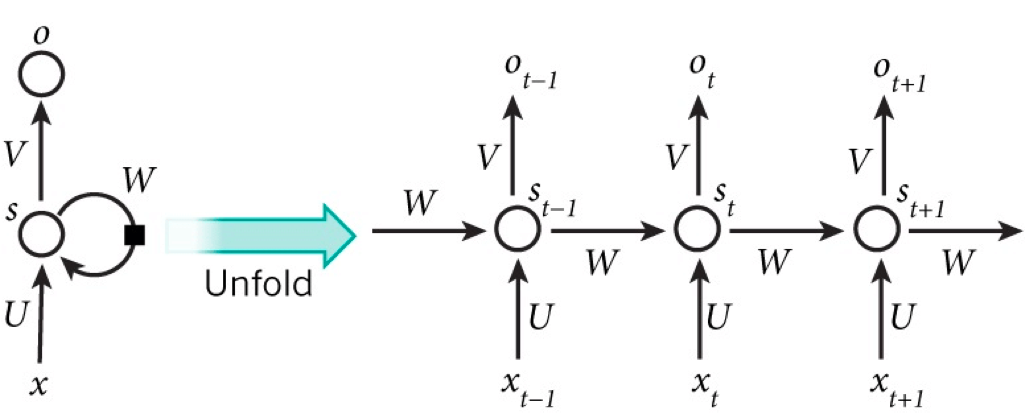
\includegraphics[width = 0.4\textwidth]{rnn-diagram}

LSTMs are a special class of RNNs augmented to better remember long-term dependencies. Within each hidden node, there is an additional cell state and a series of gates which control how much information is updated or forgotten in the cell state. These gates are depicted in the diagram below.

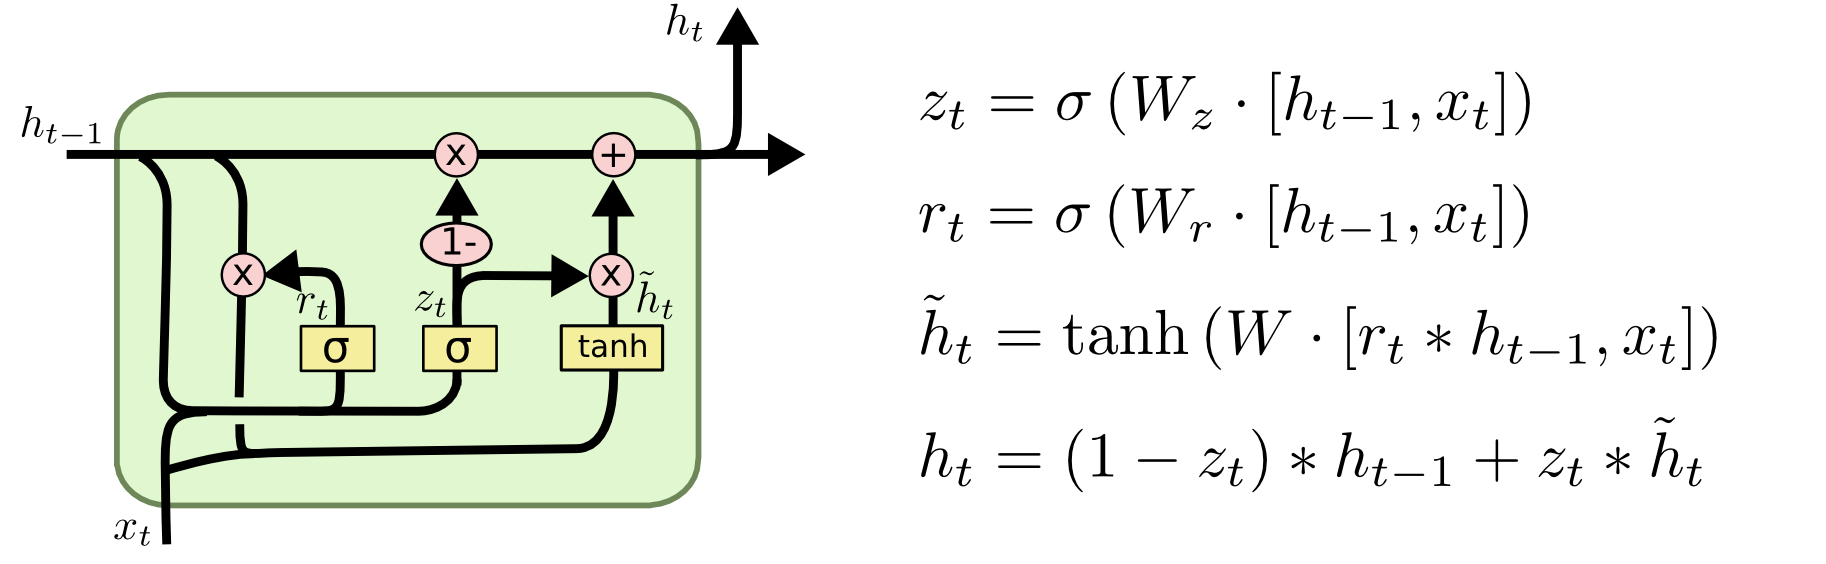
\includegraphics[width = 0.4\textwidth]{colah-lstm-diagram}

In addition, our LSTM implementation incorporate attention, which improves the ability of LSTMs to encode long-term structure. While a basic LSTM solely uses the previous output vector as input to the next cell, LSTMs with attention also take the previous $n$ output vectors as input. In other words, the model implements:
\begin{align}
u_i^t &= v^T \text{tanh}(W_1^\prime h_i + W_2^\prime c_t) \\
a_i^t &= \text{softmax}(u_i^t) \\
h_t^\prime &= \sum_{i=t-n}^{t-1} a_i^t h_i
\end{align}
Where vector $v$ and matrix $W^\prime$ are the laernable parameters. $c_t$ is the RNN's cell state at the current step, and $h_i$ are the RNN outputs from the previous $n$ steps. The model applies an mask vector called the attention mask  $a_i$ to these vectors, determining the relative weight given to each previous output. By consulting these previous output vectors, models with attention are better able to capture long-term structures like repeated notes, rhythms, and song key. \\

%------------------------------------------------

\section{Experiments}

For logistic regression, we ran 4-fold cross-validation over our training dataset, which consisted of 85\% of all of our songs. For our LSTM's, because it became too expensive to run full cross-validation, we further divided our training set into 70/15 train/validation sets and chose our hyperparameters based on performance on the  validation set.

For our logistic regression model, we ran gridsearch for the best regulation parameter C, attempting values of 0.1, 1, 10, and 100. We found that we achieved the best results with C=10.

For our simple LSTM model, we used 2 LSTM's with 128 nodes each, and a dropout of 0.2. For our attention-based LSTM model, we used 2 LSTM's with 64 nodes each. We trained each one with a batch size of 64. These parameters were chosen based on best reported results in the original attention LSTM codebase.

%------------------------------------------------


\section{Results and Evaluation}

\subsection{Prediction accuracies}
First, we evaluated our models on their ability to predict the next note of a given sequence. It is important to note that this is not necessarily indicative of model performance on the task we actually care about, which is generation. In particular, we note that humans cannot achieve anything near perfect prediction accuracy for musical sequences we have not seen before, but we are able to generate \textit{new} sequences that are melodic and exhibit sensible musical structure.

That being said, higher prediction accuracy by a model likely indicates better understanding of patterns in note sequences, chords, and most importantly, key. We compare the prediction performance of our models with 4-fold cross-validation.

We determined that our logistic regression achieves a 28.5\% accuracy  in predicting the next note on the Beethoven dataset, and an accuracy of 29.9\% for the Mozart dataset. \\

\subsection{Human evaluation}
For our primary task, we evaluated the compositions produced by our models on 16 human
evaluators. Evaluators were asked to rate the acoustic quality of the produced
compositions on a scale from 1 to 10, with a Mozart composition set as 10 to
serve as our relative best performing composition.

\begin{tabular}{|l|l|}
\hline
\textbf{Source} & \textbf{Avg. Evaluation} \\ \hline
Logistic Regr.  & 2.93                  \\ \hline
LSTM            & 5.86                  \\ \hline
Attention LSTM  & 5.31                  \\ \hline
Mozart          & 10.0                  \\ \hline
\end{tabular} \\

Both LSTM models clearly outperform our logistic regression baseline but lag behind the original Mozart composition. We are somewhat surprised that our attention LSTM fails to outperform the standard LSTM. This may indicate that attention has a limited effect on acoustic results, or it may be a result of our relatively small sample of human evaluators.

\subsection{Analysis of Samples}
We further compared the distribution of generated notes for a few samples of the logistic regression baseline and simple LSTM model.

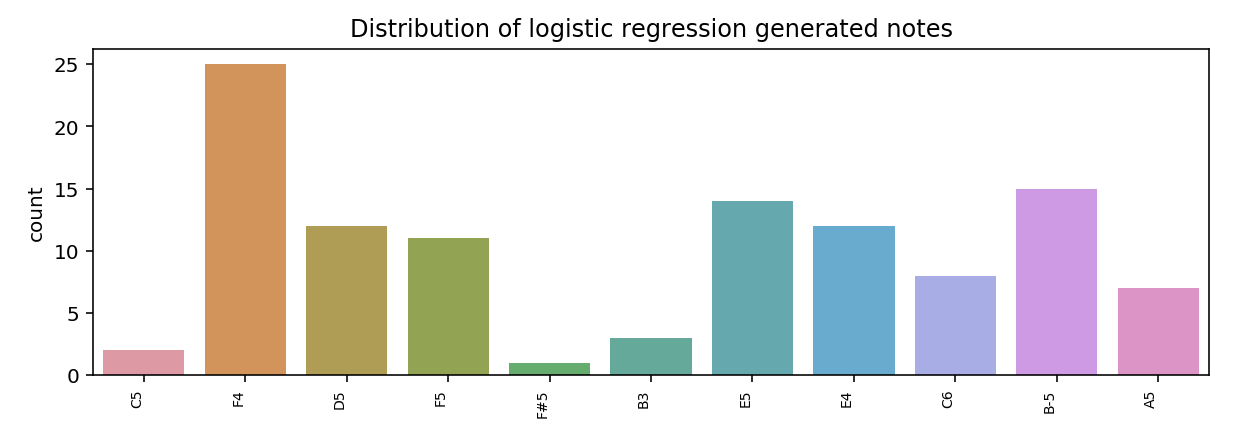
\includegraphics[width = 0.45\textwidth]{images/logreg_notes.png}

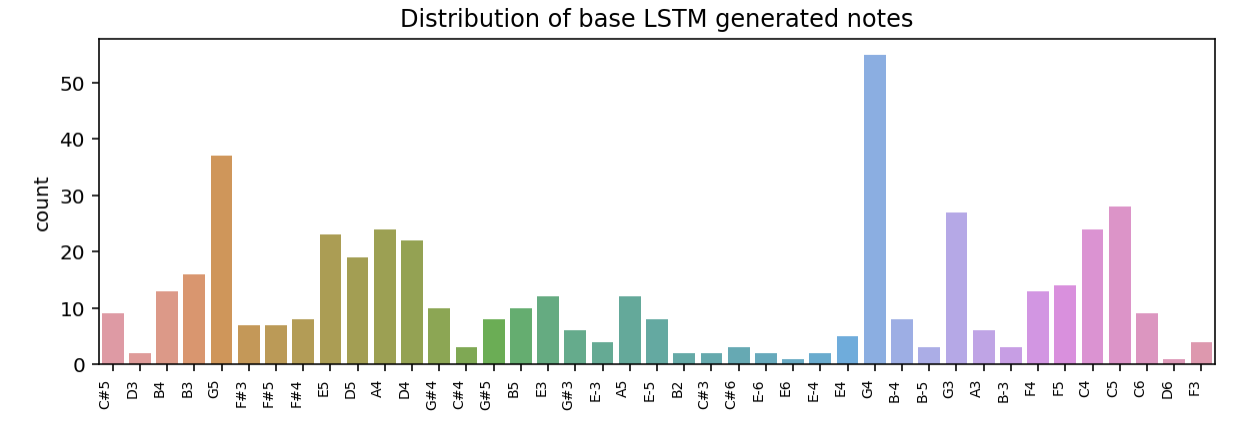
\includegraphics[width = 0.45\textwidth]{images/simple_lstm_notes.png}

As expected, both models generate a smaller range of notes than the original Beethoven samples shown earlier (although, the Beethoven samples contained more songs and thus more notes in total than the samples we are evaluating). Even so, logistic regression is notably even more limited in range, alternating among 11 different notes for 3 songs. While the vanilla LSTM is much more varied, it is similarly susceptible to repetition of single notes, with G4 being generated almost twice as often as any other note.

For comparison, we calculated the prediction accuracy that would be obtained by using a classifier that just predicts the most common note (MCN) in these output samples. The accuracies that would be achieved with this MCN predictor are reported in the table below, both for the generated outputs and the original Beethoven and Mozart pieces. \\

\begin{tabular}{|l|l|}
\hline
\textbf{Source} & \textbf{MCN Accuracy} \\ \hline
Logistic Regr.  & 22.73                 \\ \hline
LSTM            & 11.65                 \\ \hline
Beethoven       & 5.91                  \\ \hline
Mozart          & 3.23                  \\ \hline
\end{tabular} \\

As we can see, the logistic regression samples seem to have the highest frequency of their most common note. Again, while the LSTM samples only reach half that frequency for their most frequent note, both the logistic regression and LSTM samples use their most frequent note at least twice as much as the Beethoven and Mozart original compositions. Simply put, our baseline models generate outputs that heavily repeats itself, more on a note-by-note basis than on any particular melodic pattern.

\subsection{Discussion of Models}

As expected, our logistic regression baseline fails to capture long-term
structure in the training set. The heavy use of repetition can be seen in the example composition below:

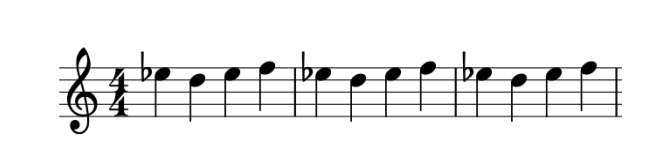
\includegraphics[width = 0.45\textwidth]{images/logreg_composition.png}

Meanwhile, the compositions generated by our LSTM models (both the regular LSTM and our attention-based LSTM) exhibit more
variation, while maintaining some long-term structure and repeated
melodies throughout the piece:

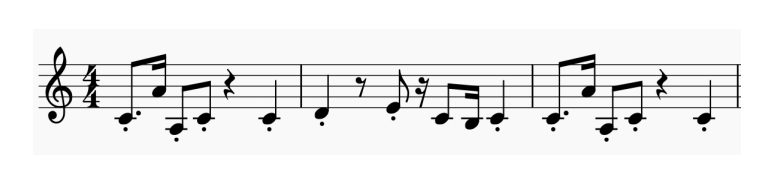
\includegraphics[width = 0.45\textwidth]{images/magenta_composition.png}

We suspect the reason LSTM's are able to perform so much better is that they have a hidden state that works as the "memory" of the network, and this hidden state is gated such that it can store and recall past signals for a long period of time. In contrast, the logistic regression model only gets the past 10 notes as an input, in no particular order or emphasis.

Furthermore, it makes sense that the attention-based LSTM outperforms the normal LSTM, especially for generating musical sequences. Notably, repetition in music often happens across 1 or 2 bars, and attention-based LSTM's allow the model to focus in on the appropriate corresponding previous hidden states at each time step. In other words, the model learns to focus on the second note of the previous melody when it is trying to generate the second note of the repeated melody.

These qualitative differences in composition align with our expectations, as well as the quantitative difference in average human
evaluation score. We conclude that LSTMs are better able to capture long-term dependencies and structure in musical compositions.


%------------------------------------------------


\section{Conclusion}

\subsection{Summary of Results}

We find that logistic regression models are unable to capture long-term patterns in music, and default to generating the most common notes or 2-4 note sequences. Meanwhile, our regular LSTM model is able to vary its generated output much more significantly, likely because its internal memory cell is able to condition on longer sequences of notes and capture greater variation within them. Finally, our attention-based LSTM model is further able to capture repetitions of simple melodies across a few bars, which is consistent with the ability of the attention mechanism to focus on important previous states.


\subsection{Future Steps}
If we had more time or resources, there are a few extensions of our current research that we would like to pursue.

First and foremost, we would like to extend our baseline models to handle and predict rhythm in addition to notes and chords. Right now, our attention-based LSTM model is able to predict "rest" or "hold" events, but our regular LSTM and logistic regression baselines are lacking in those features. We would have liked to add those in for a better comparison of generated music samples.

We would also like to generalize beyond just piano melodies and explore generation with
other instruments, percussions, or electronic sounds. In addition, we hope to
explore ways to generate multiple notes per time step, and experiment with generative models such as variational auto-encoders to further improve our time-structure
representation.


\section{Contributions}

Eric handled data preprocessing to extract note sequences from MIDI files, and trained the logistic regression baseline to compose. Joyce trained the standard LSTM model to compose, and performed much of the data visualization throughout the paper. Sam trained and generated compositions with the attention-based LSTM. All team members contributed to sourcing human evaluators and writing the final paper.


%----------------------------------------------------------------------------------------
%   REFERENCE LIST
%----------------------------------------------------------------------------------------

%Sets the bibliography style to UNSRT and imports the
%bibliography file "samples.bib".
\bibliographystyle{unsrt}
\bibliography{ref}

%----------------------------------------------------------------------------------------

\end{document}

%%% Local Variables:
%%% mode: latex
%%% TeX-master: t
%%% End:
